%% Bemærk:
%%          Resten af rapporten følger en stil hvor indledninger skrives
%%          med \sffamlily-typen. Denne stil bør også følges her.
%%
{\sffamily
I dette sektion vil vi teste den naive løsning. ved at se om den sortere
de rigtige regioner væk og om løsningen opføre sig på samme måde som vi
har håbet på. Det vil vi gøre ved ført at se på nogle fabrikeret test
billeder, får at se om den naive løsning virker efter meningen og
bagefter vil vi teste på malerierne for at se om den naive løsning kan
bruges i praktisk.
}
  
\subsection{Afprøvning på testbilleder}
Vi vil teste på de samme testbilleder som i sideste afsnit, samt et nyt
testbilleder som blev brugt i forklaringen af den naive metodes, de fire
billeder som vi har valt at test kan se i afsnit \ref{region_detektor}
og billedet \ref{naiv_masse_original} hvor en grån kasse rundt om en
region, betyder at den er valt til at ligge i det gyldne snit af den
naive metode. 

Det første billedet \ref{naiv_blob1}, har fem regioner og hvor tre af
dem blev fundet af reginon detektoren, vores naive løsning har så
sorteret baggrundens regionen og den øverste region i snitte vær, da de
begge krydser marginer og derfor ikke overholder definition
\ref{} . 

\begin{figure}[!h]
	\begin{center}
        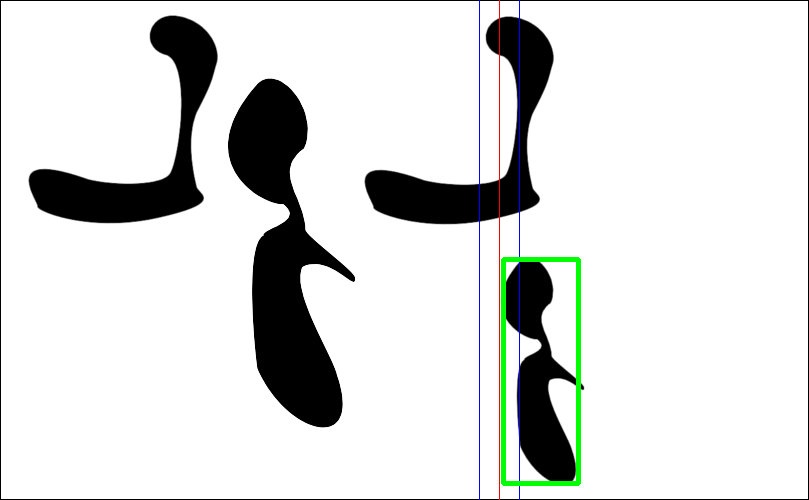
\includegraphics[angle=0,width=0.55\textwidth]{afsnit/afprovning/billeder/naive_losning/naiv_blob1.png}
	\end{center}       
	\caption{Naive algoritme finder en ud af fem regioner}	
	\label{naiv_blob1}
\end{figure}

Det andet billedet \ref{naiv_blob2}, er alle blevet sorteret vær, også
den lille, da den er for lille, derfor ikke overholder definition
\ref{def_interessant} b. 

\begin{figure}[!h]
	\begin{center}
       	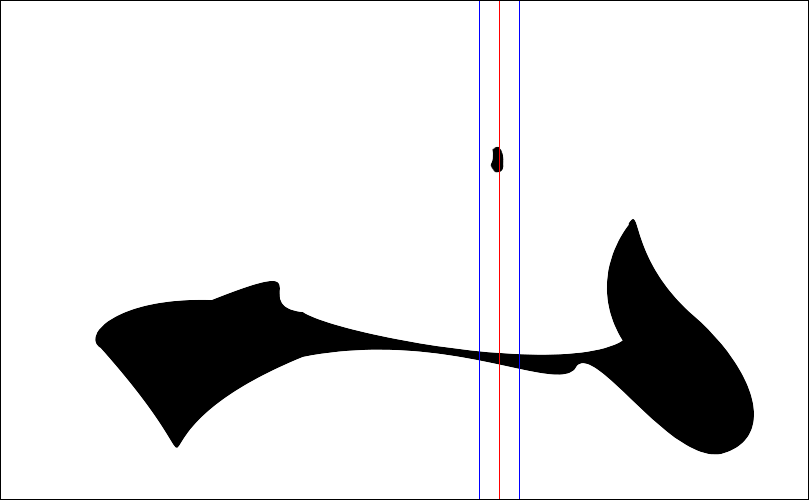
\includegraphics[angle=0,width=0.55\textwidth]{afsnit/afprovning/billeder/naive_losning/naiv_blob2.png}
	\end{center}
	\caption{Værgen den lille region eller den store er fundet} 
   	\label{naiv_blob2}
\end{figure}

I test billedet \ref{naive_hoisont1}, sortere algoritmen
himlen fra, da den krydser margin lidt, men tager jorden med. 

\begin{figure}[!h]
	\begin{center}
       	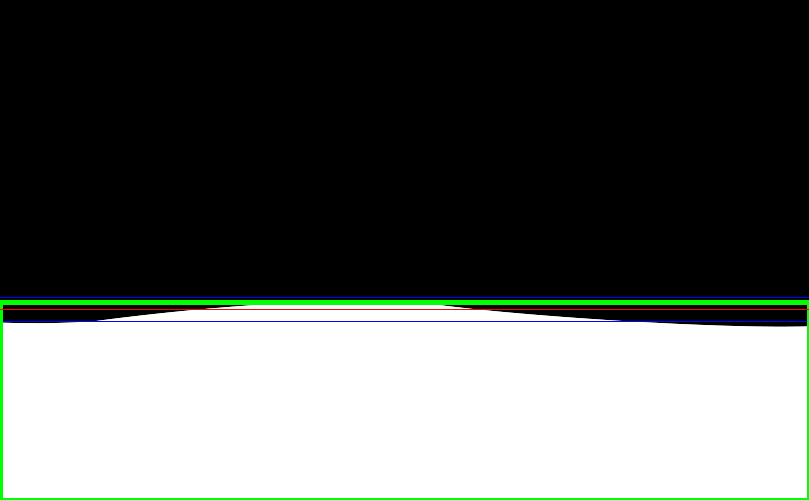
\includegraphics[angle=0,width=0.55\textwidth]{afsnit/afprovning/billeder/naive_losning/naiv_hoisont1.png}
	\end{center}
	\caption{Kun den nederste højrisondt er fundet} 
   	\label{naive_hoisont1}
\end{figure}

\clearpage

\subsection{Afprøvning på malerier}
Vi afprøver den naive algoritme på seks malerier, først på tre malerier,
hvor regions detektoren virker efter vores hensigt og så på ter
malerier, hvor region detektoren ikke virker. Beskrivelsen af hvad der
sker i billedet vil står i caption


\begin{figure}[h!!]
	\begin{center}
		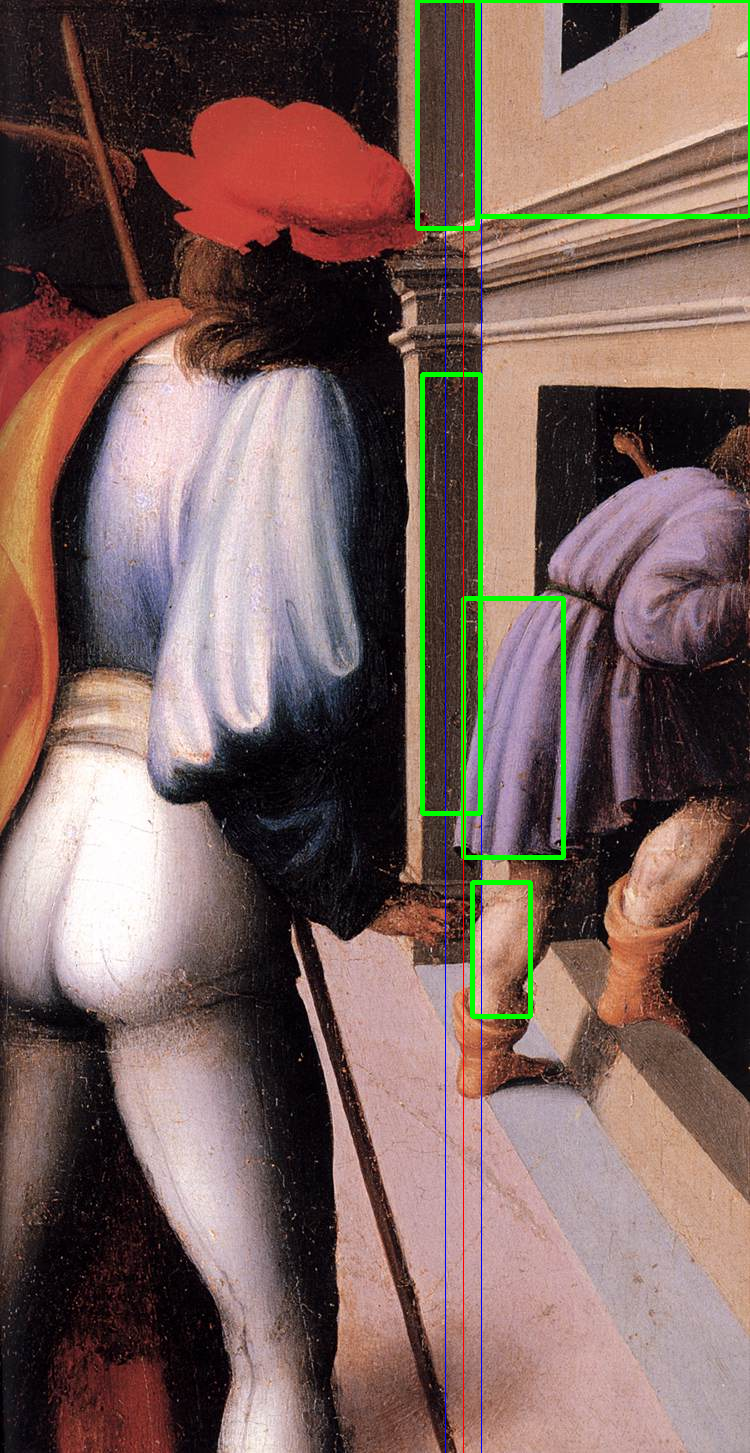
\includegraphics[scale=0.3,angle=0]{afsnit/afprovning/billeder/naive_losning/naiv_kfarver_sdetaljer.png}
	\end{center}
	\caption[]{Fem ud af de seks store regioner fra figur
	\ref{GRD_virker1} valt til at ligge i snittet, skoene er få små til
	at blive taget i betragtning}
	\label{naiv_kfarver_sdetaljer}
\end{figure}

\begin{figure}[h!!]
	\begin{center}
		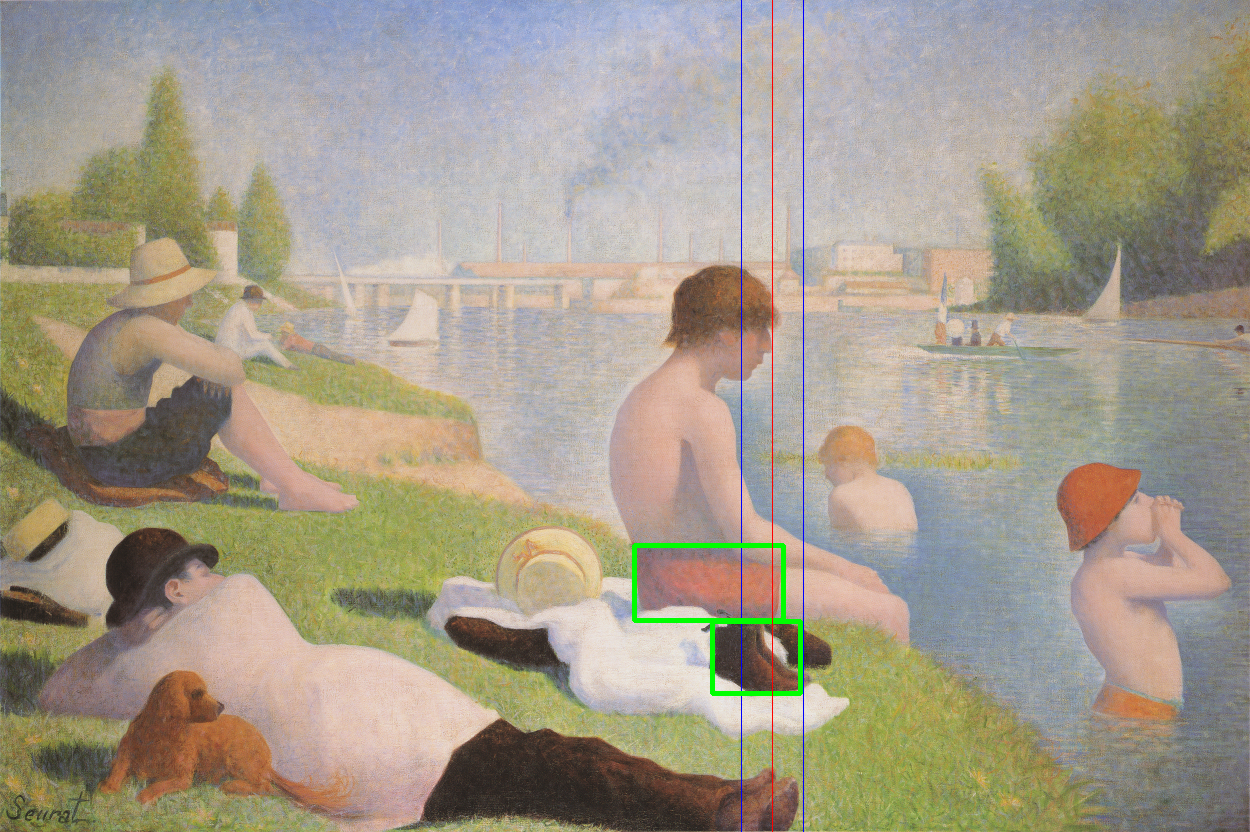
\includegraphics[scale=0.3,angle=0]{afsnit/afprovning/billeder/naive_losning/naiv_mfarver_mdetaljer.png}
	\end{center}
	\caption[]{Bukserne og skoene er tager med af den naive løsning, men
	drengen er sorteret væk da har krydser snittet}
	\label{naiv_mfarver_mdetaljer}
\end{figure}

\begin{figure}[h!!]
	\begin{center}
		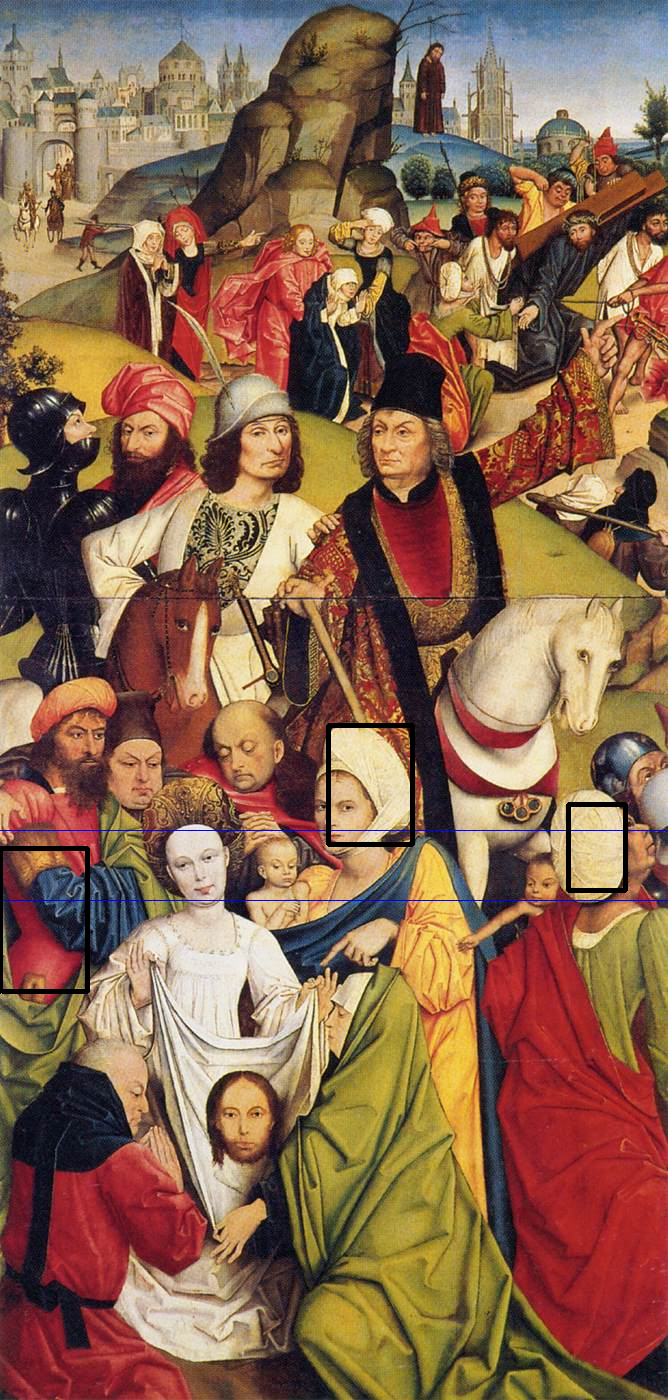
\includegraphics[scale=0.3,angle=0]{afsnit/afprovning/billeder/naive_losning/naiv_kfarver_kdetaljer.png}
	\end{center}
	\caption[]{Et billedet med mange hoder i snittet, hvor to af dem
	bliver godtaget af den naive metode til at ligger i snittet, en
	trøje bliver desværre også taget med. Navn: Christ Carrying the
	Cross. År: 1480. Af: Bosch Hieronymus}
	\label{naiv_kfarver_kdetaljer}
\end{figure}

\begin{figure}[h!!]
	\begin{center}
		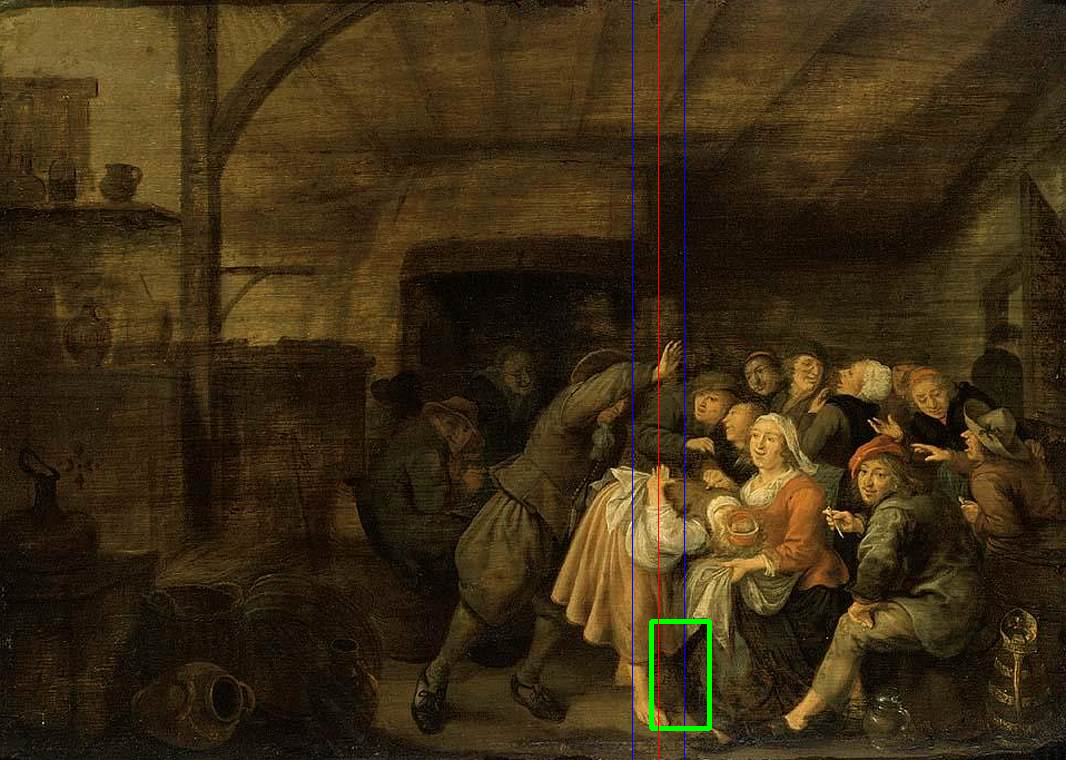
\includegraphics[scale=0.3,angle=0]{afsnit/afprovning/billeder/naive_losning/naiv_virker_ikke1.png}
	\end{center}
	\caption[]{Mallerie hvor region detektor ikke virker, den naive
	løsning godtager tager en region som ligger helt forkert. Navn:
	Peasants in an Inn Playing "La Main Chaude". År: Ukendt. Af:
	Molenaer, Jan Miense.}
	\label{naiv_virker_ikke1}
\end{figure}

\begin{figure}[h!!]
	\begin{center}
		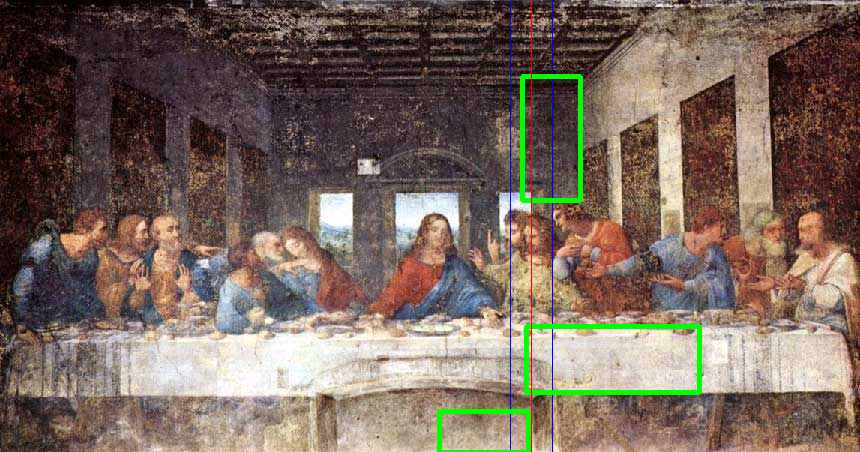
\includegraphics[scale=0.3,angle=0]{afsnit/afprovning/billeder/naive_losning/naiv_virker_ikke2.png}
	\end{center}
	\caption[]{Tre regioner bliver godtaget, selv om de ikke er særlige
	intresante }
	\label{naiv_virker_ikke2}
\end{figure}

\begin{figure}[h!!]
	\begin{center}
		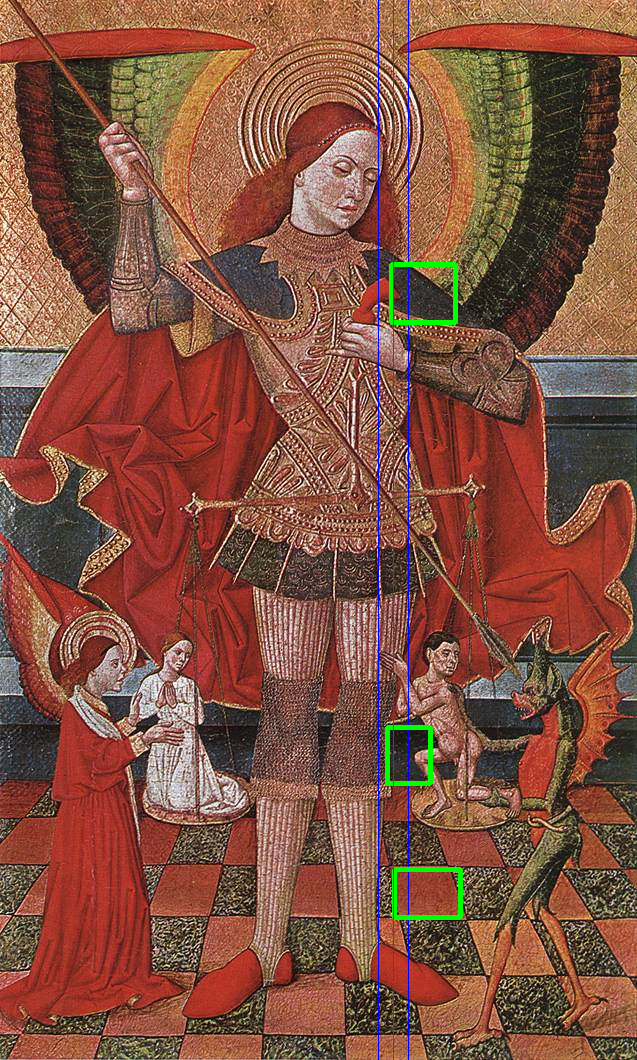
\includegraphics[scale=0.3,angle=0]{afsnit/afprovning/billeder/naive_losning/naiv_virker_ikke3.png}
	\end{center}
	\caption[]{Der bliver fundet tre region, hvor kun en af dem passer
	på en ting i billedet}
	\label{naiv_virker_ikke3}
\end{figure}
\clearpage

For at give et bedre indblik på hvor mange regioner vi mener er
interessante og hvor mange der er falske positiver, har vi optalt dem på
de samme ni malerier som i tærskelværdi afprøvningen. I tabel
\ref{naiv_good} kan ses antallet af interessante regioner og i tabel
\ref{naiv_bad} kan ses antallet af falske positive. Der bliver fundet 12
interessante regioner og 10 falske positive, det vil sige at der er $20
\%$ flere interessante region end falske.

\begin{table}[H]
    \centering
    \begin{tabular}{|c|l|l|l|}
			\hline
            & Kraftige farver & Medium farver & Svage farver \\\hline
		Mange detaljer	& 2 & 0 & 7 \\\hline
        Medium detaljer  & 1 & 0 & 0 \\\hline
        Få detaljer     & 1 & 0 & 1 \\\hline
    \end{tabular}
    \caption[]{Tabel over antal interessant regioner fundene i ni test malerier.}
    \label{naiv_good}
\end{table}

\begin{table}[H]
    \centering
    \begin{tabular}{|c|l|l|l|}
			\hline
            & Kraftige farver & Medium farver & Svage farver \\\hline
		Mange detaljer	& 3 & 0 & 0 \\\hline
        Medium detaljer  & 0 & 3 & 0 \\\hline
        Få detaljer     & 1 & 3 & 0 \\\hline
    \end{tabular}
    \caption[]{Tabel over antal falske positiver i ni test malerier.}
    \label{naiv_bad}
\end{table}

\subsection{Konklusion}
Det naive løsning virker efter intentionen på testbillederne, men i
praktisk finder den mange regioner som vi helst
vil være for uden som f.eks i maleriet \ref{naiv_virker_ikke3}. 
Ved disse testbilleder findes der altså kun $20\%$ flere interessante
regioner, som vi finder korrekt detekteret end falske positiver. 
Denne overvægt betyder at billederne er illustrative for det vi prøver
at finde, det er sagt med den forudsætning at det fulde billedkorpus
deler samme egenskaber som de ni testbilleder.
